\chapter{Contexte Général et Étude de l'Existant}

\section{Introduction}
Tout projet informatique naît d'un besoin réel identifié au sein d'une organisation.
Ce chapitre est consacré à la présentation détaillée de l'organisme d'accueil, Naftal,
de son Système d'Information et du département au sein duquel notre projet a été réalisé.
Nous y exposerons ensuite l'étude de l'existant afin d'en dégager les limites et de justifier
la solution logicielle proposée.

\section{Présentation de l'Organisme d'Accueil : Naftal}

\subsection{Aperçu Historique}
Le nom \textbf{NAFTAL} est formé de deux racines : \textit{NAFT} (pétrole en arabe) et
\textit{AL} (Algérie), symbolisant sa mission nationale. L'entreprise a été créée par le décret
N°~80-101 du 09~avril~1980, initialement sous la tutelle de Sonatrach pour les activités de
raffinage et de distribution des produits pétroliers (ERDP). Suite à la séparation des activités
de raffinage et de distribution par le décret N°~80-187 du 27~août~1987, deux entités
distinctes ont vu le jour : \textbf{NAFTAC} (raffinage) et \textbf{NAFTAL} (distribution).
Depuis le 18~avril~1998, Naftal est devenue une \textbf{Société Par Actions (SPA)}, filiale
à 100\% de Sonatrach, avec un capital social évalué à \textbf{15,65 milliards de dinars}~\cite{ingrachen2016}.

\subsection{Missions et Activités}
La mission principale de Naftal est la \textbf{distribution et la commercialisation des
produits pétroliers} sur le marché national algérien. Elle intervient également dans :
\begin{itemize}
    \item L'enfûtage et la commercialisation des GPL (Gaz de Pétrole Liquéfié) ;
    \item Le transport, le stockage et la formulation des bitumes ;
    \item L'organisation et le développement du réseau de distribution national ;
    \item Les activités internationales et partenariats.
\end{itemize}

\subsection{Envergure et Moyens}
Pour assurer ses missions à l'échelle nationale, Naftal dispose de moyens considérables~\cite{ingrachen2016} :
\begin{itemize}
    \item Un effectif de \textbf{30~000 agents} dont 25~000 permanents (2~800 cadres,
    7~500 agents de maîtrise) ;
    \item \textbf{65} centres et dépôts de distribution de carburants (CLP) ;
    \item \textbf{3~600} véhicules de distribution et 840~km de canalisations opérationnelles ;
    \item Un réseau de \textbf{1~846 stations-service} sur l'ensemble du territoire ;
    \item \textbf{49} dépôts relais de stockage GPL et \textbf{1~100} points de vente GPL.
\end{itemize}

\subsection{Organisation Structurelle}
Naftal est organisée selon une structure fortement hiérarchisée, basée sur le principe de
la \textbf{spécialisation par ligne de produits} et la décentralisation des structures
opérationnelles~\cite{meghari2014}. Elle comprend :
\begin{itemize}
    \item Une \textbf{Direction Générale} pilotée par un PDG ;
    \item Des \textbf{Directions Exécutives}, chargées de la stratégie et du pilotage ;
    \item Des \textbf{Directions Centrales}, centres d'expertise (audit, R\&D, DCSI) ;
    \item Cinq \textbf{Branches opérationnelles} : Carburants, Commercialisation, GPL,
    Lubrifiants-Pneumatiques-Bitumes, et Activités Internationales.
\end{itemize}

\begin{figure}[H]
  \centering
  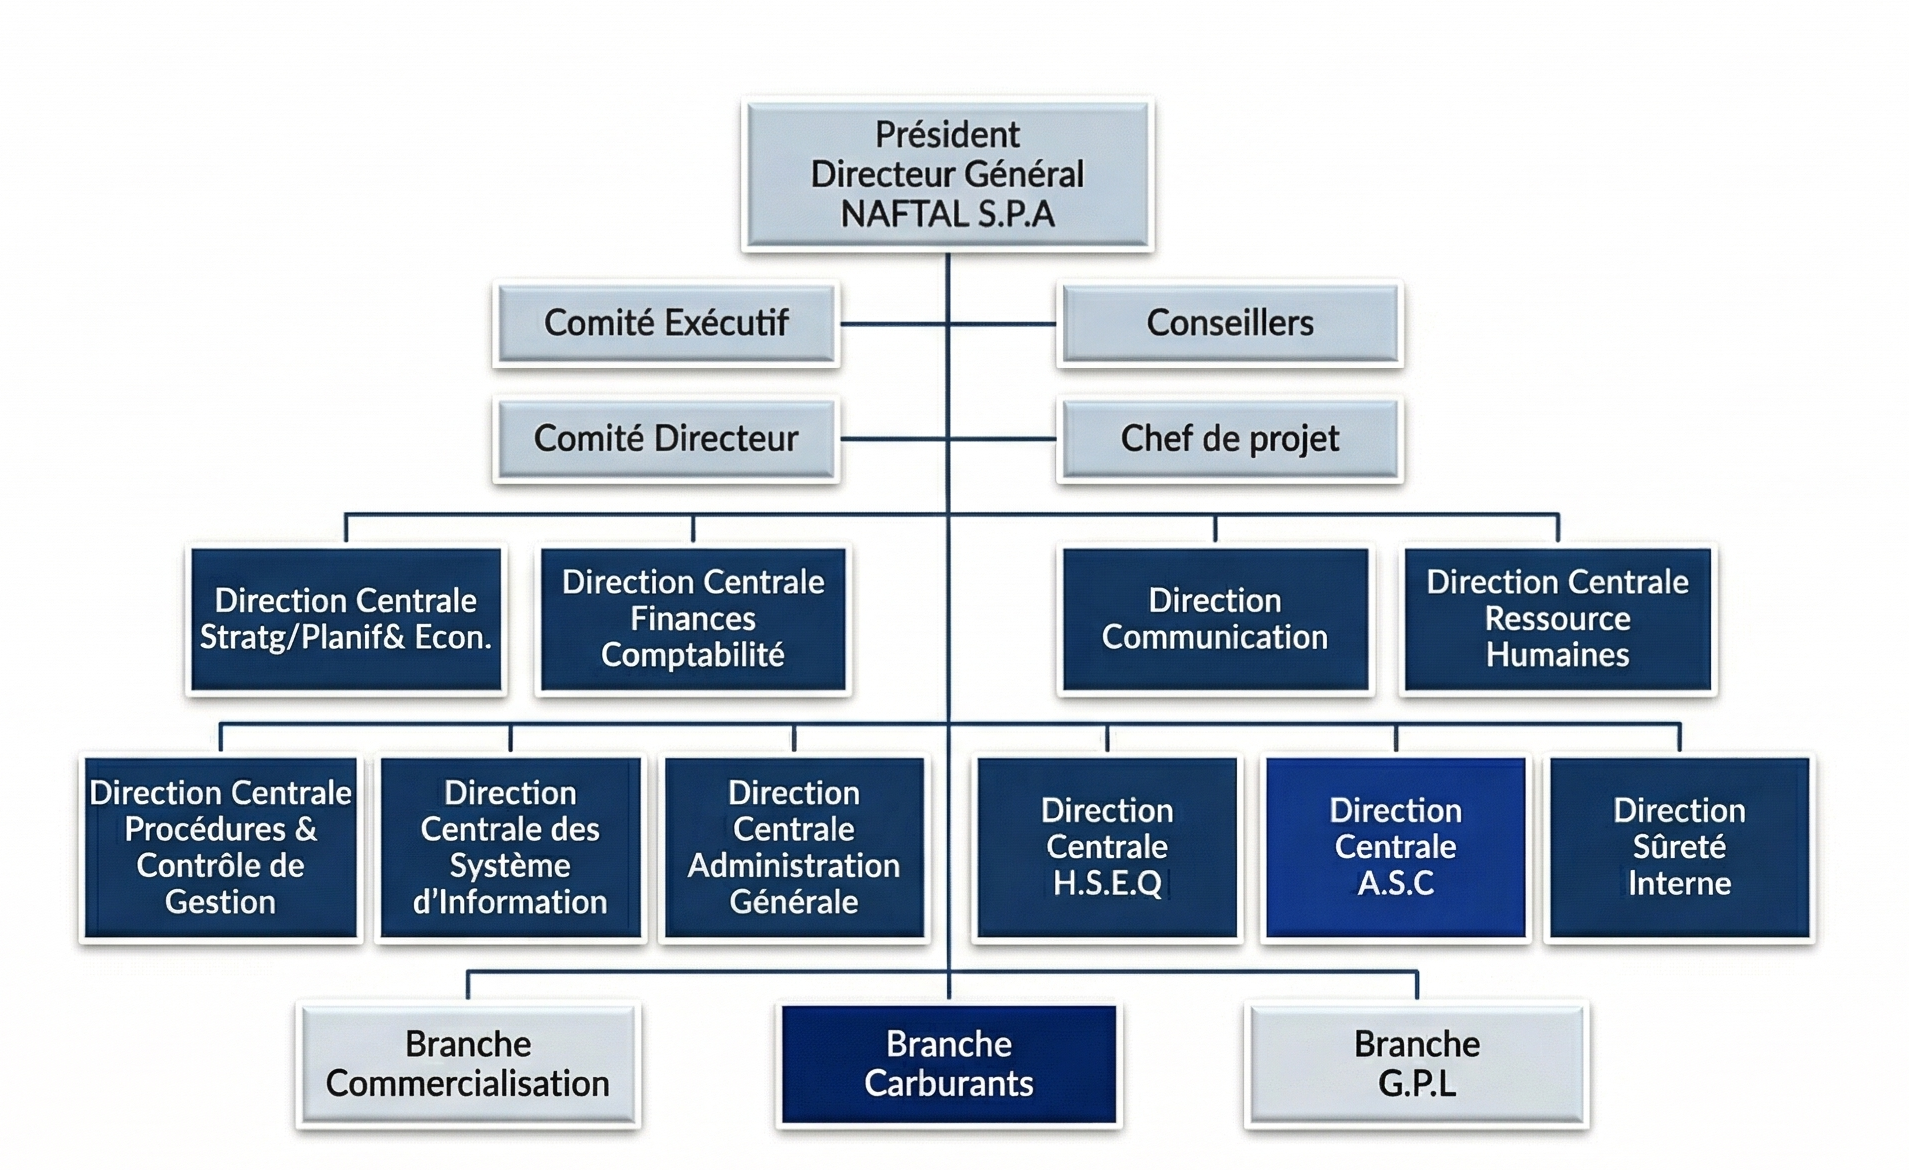
\includegraphics[width=0.90\textwidth]{figures/organigramme_naftal}
  \caption{Organigramme général de Naftal SPA
           (Source : documents internes Naftal)}
  \label{fig:organigramme_naftal}
\end{figure}

\subsection*{Les onze Directions Centrales}
La société NAFTAL est dotée de onze (11) Directions Centrales qui constituent
ses structures fonctionnelles de haut niveau~\cite{ingrachen2016} :

\begin{itemize}
    \item \textbf{DCSPE} — Stratégie, Planification et Économie.
    \item \textbf{DCF} — Finances.
    \item \textbf{DCRH} — Ressources Humaines.
    \item \textbf{DCSI} — Systèmes d'Information \textbf{(direction concernée
    par notre projet GIA)}.
    \item \textbf{DCCGP} — Contrôle de Gestion et Procédures.
    \item \textbf{DRD} — Recherche et Développement.
    \item \textbf{DCA} — Audit.
    \item \textbf{DCHSEQ} — Hygiène, Sécurité, Environnement et Qualité.
    \item \textbf{DCASC} — Affaires Sociales et Culturelles.
    \item \textbf{DCSIE} — Sûreté Interne.
    \item \textbf{DCAG} — Administration Générale.
\end{itemize}

La section suivante présente en détail la \textbf{DCSI}, dont relève directement le Groupe
Informatique de la Branche Carburants, cadre opérationnel de notre projet.

\subsection{Macrostructure et grands équilibres institutionnels}
Dans un contexte marqué par l'adaptation au cadre légal et par une concurrence accrue, Naftal
a structuré son organisation autour de la spécialisation par activité. La macrostructure
(actualisée notamment dans les années 2000) distingue~\cite{meghari2014} :
\begin{itemize}
    \item la \textbf{Direction générale} et le \textbf{staff exécutif}, chargés des orientations,
    de la coordination globale, du pilotage, du management et de la veille stratégique ;
    \item les \textbf{structures fonctionnelles} : directions exécutives, directions centrales
    et directions de soutien au siège ;
    \item les \textbf{structures opérationnelles} : branches d'activités (Carburants,
    Commercialisation, GPL, Lubrifiants--Pneumatiques--Bitumes, Activités internationales et
    partenariats).
\end{itemize}

Les \textbf{directions exécutives} assurent, chacune dans son domaine, l'anticipation des
tendances, la conception des instruments de pilotage et de contrôle, le management stratégique,
l'assistance aux structures opérationnelles et la définition de la politique générale. Les
\textbf{directions centrales} constituent des centres d'expertise (recherche et développement,
audit, procédures et contrôle de gestion, communication, HSE, sûreté, \textbf{systèmes
d'information}, etc.). Les \textbf{directions de soutien} gèrent l'administration du siège.
Cette architecture explique la place centrale de la DCSI : elle relève des structures fonctionnelles
de haut niveau tout en servant l'ensemble des branches.

\subsection{Le Système d'Information de Naftal}
Naftal est pionnière dans l'informatisation de sa gestion en Algérie. Son SI est
articulé autour de plusieurs composantes clés gérées par la
\textbf{Direction Centrale des Systèmes d'Information (DCSI)}~\cite{ssiouani2010} :
\begin{itemize}
    \item \textbf{NAFT COM} : système de gestion commerciale (facturation, ventes, stocks) ;
    \item \textbf{WINCANAL} : logiciel de comptabilité analytique ;
    \item \textbf{NAFT GD} : gestion des stations-service en Gestion Directe ;
    \item \textbf{Un réseau Intranet} (VPN 2 Mb/s) reliant la Direction Générale, les
    Branches (GPL, Carburants, Commercialisation) et les Districts sur tout le territoire.
\end{itemize}
La DCSI est responsable de la mise en place, du suivi technique, gestionnaire et
stratégique de ce SI. Comme l'a démontré l'étude de Meghari~\cite{meghari2014},
l'évaluation de la performance de cette fonction révèle un besoin croissant en outils
de support et de traçabilité des incidents.

\section{La DCSI : missions, tâches et organisation interne}
La \textbf{Direction centrale des systèmes d'information (DCSI)} est la structure corporate
chargée de la fonction SI~\cite{ssiouani2010,meghari2014}. Créée dans le cadre des
réorganisations du groupe (historiquement issue du rapprochement avec les structures «\,systèmes
d'information et procédures\,»), elle relève aujourd'hui de la direction générale. Ses
\textbf{missions} affichées couvrent notamment :
\begin{itemize}
    \item organiser la migration des systèmes existants vers des plateformes plus performantes ;
    \item déployer des progiciels et outils modernes (ERP, analyse de données, aide à la décision).
\end{itemize}

Ses \textbf{tâches et responsabilités} opérationnelles, telles que décrites dans les documents
d'organisation de l'entreprise et synthétisées dans la littérature de cas Naftal~\cite{meghari2014},
incluent entre autres :
\begin{itemize}
    \item doter l'entreprise d'une infrastructure de communication (réseau étendu intégrant les
    structures de la société) ;
    \item déployer des réseaux locaux jusqu'aux centres de distribution et de stockage ;
    \item veiller à la cohérence de l'environnement informatique (technologies et ressources) ;
    \item assurer sécurité et confidentialité des systèmes d'information ;
    \item mettre en œuvre des progiciels couvrant les fonctions de la société ;
    \item constituer et superviser les groupes chargés de la conduite de projets (analyse,
    conception, développement, formation, déploiement, consolidation, assistance) ;
    \item produire périodiquement des tableaux de bord alimentés par les données de gestion.
\end{itemize}

\subsection{Départements de la DCSI et domaines d'intervention}
La DCSI s'articule en départements spécialisés ; le tableau~\ref{tab:dcsi_depts} en reprend la
logique fonctionnelle (effectifs indicatifs issus des études de terrain disponibles à l'époque des
travaux de référence — ils sont donnés à titre \textbf{illustratif} et peuvent avoir évolué).

\begin{longtable}{@{}p{3.6cm}p{1.1cm}p{9.3cm}@{}}
\caption{Vue synthétique des départements de la DCSI Naftal (d'après organigramme et fiches de
mission documentés dans la littérature de cas~\cite{meghari2014})\label{tab:dcsi_depts}} \\
\toprule
\textbf{Département} & \textbf{Eff.} & \textbf{Profils et responsabilités principales} \\
\midrule
\endfirsthead
\multicolumn{3}{c}{\tablename\ \thetable{} — \textit{suite}} \\
\toprule
\textbf{Département} & \textbf{Eff.} & \textbf{Profils et responsabilités principales} \\
\midrule
\endhead
\midrule
\multicolumn{3}{r}{\textit{Suite page suivante}} \\
\endfoot
\bottomrule
\endlastfoot
Systèmes Back Office &
9 &
Chefs de projet administration systèmes, sécurité informatique : coordination avec les autres
départements, implémentation et optimisation des SGBD ; confidentialité, intégrité et disponibilité
des données ; sécurisation et gestion des données hébergées sur les supports concernés ;
supervision de groupes projet (analyse à assistance) ; production de tableaux de bord ;
assainissement du référentiel de données et maintien de son unicité pour la cohérence des
interfaces inter-systèmes. \\
\midrule
Systèmes opérationnels &
11 &
Chefs de projet, intégrateurs : planification des systèmes de valorisation et publication des
indicateurs ; participation aux cahiers des charges et analyse d'offres web, décisionnelles ou
mixtes ; intégration des solutions web et décisionnelles alignées sur la politique
d'informatisation. \\
\midrule
Solutions Web \& systèmes décisionnels &
10 &
Chefs de projet web et décisionnel : même logique d'intégration et d'alignement stratégique sur
les besoins de publication d'indicateurs et de portails. \\
\midrule
Traitements informatiques &
10 &
Techniciens transfert de données, traitement, chargés d'études : organisation des ressources pour
les traitements ; maintien en condition des moyens matériels ; cahiers des charges de
renouvellement et d'extension des équipements de traitement. \\
\midrule
Support \& réseaux informatiques &
13 &
Ingénieurs hardware/système, techniciens, chargés d'études : études d'installation réseau ; fiches
techniques équipements ; installation et maintenance ; élaboration et diffusion des procédures
d'utilisation des ressources informatiques. \\
\midrule
Archives centrales &
13 &
Cadres d'études, archivistes, opérateurs : inventaire et situation des archives à l'échelle
société ; mise en place des structures d'archivage ; formation des archivistes ; encadrement du
personnel concerné. \\
\end{longtable}

Les \textbf{branches} et directions métiers — dont la Branche Carburants — constituent les
principaux \emph{clients internes} du SI. Le projet GIA ne se substitue pas à la DCSI : il
complète, à l'échelle de la Branche Carburants, la \textbf{gestion de la relation utilisateurs} et
la \textbf{gestion des anomalies applicatives}, en accord avec les missions globales décrites
ci-dessus.

\section{Environnement du secteur et analyse SWOT de Naftal}
Le marché algérien de la distribution des produits pétroliers connaît une \textbf{évolution
réglementaire continue}, des \textbf{normes HSE} de plus en plus exigeantes, l'arrivée
d'\textbf{acteurs privés} dynamiques aux méthodes différenciées, une \textbf{diversification}
des besoins, le renforcement des infrastructures nationales (routes, ports, fer) et des
\textbf{consommateurs plus exigeants}. La politique énergétique vise à améliorer la performance du
secteur. Naftal, leader historique, doit maintenir la disponibilité de ses produits sur tout le
territoire, y compris dans des conditions difficiles~\cite{ingrachen2016,meghari2014}.

L'\textbf{ouverture du marché} aux opérateurs nationaux et étrangers accroît la concurrence sur
la distribution et la commercialisation. Pour préserver sa position, Naftal doit combiner
exploitation judicieuse du SI et \textbf{efforts d'adaptation} continus (compétitivité, qualité,
performance). L'environnement combine mondialisation, évolution du cadre commercial et, sur le
plan interne, un réseau de stations dense mais perçu parfois comme perfectible sur le plan de
l'offre non-carburant et de la culture sécurité — thèmes déjà soulignés dans les analyses
stratégiques du groupe~\cite{meghari2014}.

Le tableau~\ref{tab:swot} reprend une \textbf{matrice SWOT} structurée comme dans les études de cas
publiées sur Naftal : elle synthétise des \emph{forces} et \emph{faiblesses} internes ainsi que
des \emph{opportunités} et \emph{menaces} externes. Elle sert ici de \textbf{cadrage} ; les
formulations s'appuient sur la documentation interne et les travaux académiques disponibles, sans
reprendre une enquête primaire spécifique au présent mémoire.

\begin{table}[H]
\centering
\footnotesize
\begin{tabularx}{\textwidth}{@{}XX@{}}
\toprule
\textbf{Forces} & \textbf{Faiblesses} \\
\midrule
\begin{minipage}[t]{\linewidth}
\vspace{0pt}
\begin{itemize}
    \item Appartenance à Sonatrach, groupe pétrolier international.
    \item Réseau de stations-service historique et expérience de terrain.
    \item Implantation nationale et deuxième entreprise du pays en termes d'envergure.
    \item Infrastructures de transport et de stockage importantes.
    \item Gamme de produits diversifiée ; capacités de développement.
\end{itemize}
\end{minipage}
&
\begin{minipage}[t]{\linewidth}
\vspace{0pt}
\begin{itemize}
    \item Risques liés à une culture de « monopole » encore présente dans les représentations.
    \item Stations : déficit relatif de commodités modernes et d'activités non-fuel.
    \item Prestations de service parfois jugées insuffisantes ; marketing encore embryonnaire.
    \item Culture hygiène-sécurité perfectible ; stratégie parfois en décalage avec les tendances.
    \item Exploitation du SI de communication et du potentiel du réseau à renforcer.
    \item Veille technologique sur certains produits à consolider.
\end{itemize}
\end{minipage}
\\
\midrule
\textbf{Opportunités} & \textbf{Menaces} \\
\midrule
\begin{minipage}[t]{\linewidth}
\vspace{0pt}
\begin{itemize}
    \item Autoroute Est--Ouest et grands chantiers d'infrastructure.
    \item Programmes de rénovation et modernisation du parc stations.
    \item Partenariats ou sous-traitance sur activités non-fuel.
    \item Croissance de la consommation nationale.
\end{itemize}
\end{minipage}
&
\begin{minipage}[t]{\linewidth}
\vspace{0pt}
\begin{itemize}
    \item Entrée imminente ou effective de nouveaux concurrents.
    \item Attentes clients élevées sur la qualité produits/services.
    \item Marché très concurrentiel ; formats de stations innovants chez les rivaux.
    \item Partenariats concurrents déjà établis sur les segments clés (non-fuel).
    \item Pratiques commerciales plus agressives des nouveaux entrants.
    \item Évolution du cadre législatif régissant distribution et commercialisation.
\end{itemize}
\end{minipage}
\\
\bottomrule
\end{tabularx}
\caption{Analyse SWOT de Naftal (synthèse documentaire, d'après~\cite{meghari2014})}
\label{tab:swot}
\end{table}

Cette analyse révèle une faiblesse structurelle directement adressée par notre projet : l'absence
d'outils de traçabilité du support applicatif. Un incident non documenté constitue une menace
opérationnelle réelle, pouvant paralyser l'approvisionnement d'une station-service ou bloquer la
saisie dans \texttt{NAFT\_COM}. La plateforme GIA s'inscrit donc dans une logique de réduction des
risques internes identifiés par cette analyse.

\noindent\textit{Illustration perceptive.} Le réseau de stations peut être perçu comme ne répondant
pas pleinement aux attentes clients ; des tensions sur la disponibilité de certaines gammes
(lubrifiants, pneumatiques) et sur la culture sécurité sont signalées dans la littérature de cas.
Naftal est alors incitée à renforcer notoriété, image, communication sur l'expérience, l'écoute,
les services, l'environnement et l'expertise des équipes~\cite{meghari2014} — dimensions où le
\textbf{SI et le support applicatif} jouent un rôle d'enablement.

\section{Présentation du Cadre du Projet : Branche Carburants}
Notre projet s'est déroulé au sein du \textbf{Groupe Informatique de la Branche
Carburants}, basé à Dar El Beida. La Branche Carburants est chargée des activités
d'approvisionnement, de stockage et de livraison des carburants (Aviation, Marine et Terre).
Elle supervise notamment \textbf{28 centres aviation}, \textbf{6 centres marine} et
\textbf{24 dépôts carburants terre} répartis sur le territoire national~\cite{ingrachen2016}.
Pour fonctionner, ce réseau complexe s'appuie sur un parc informatique important dont la
maintenance incombe au Groupe Informatique.

\section{Cadre méthodologique de l'étude du besoin}
La démarche suivie pour ce projet de fin d'études s'inspire des approches qualitatives usuelles
dans les organisations : \textbf{entretiens et échanges} avec le Groupe Informatique et la
Direction Informatique, \textbf{analyse du cahier des charges} validé, \textbf{observation} du
fonctionnement du support existant (téléphone, messagerie non structurée) et \textbf{revue
documentaire} (travaux sur le SI Naftal, DCSI, performance de la fonction
SI~\cite{ssiouani2010,meghari2014,ingrachen2016}). Cette combinaison est comparable, à plus petite
échelle, aux investigations décrites dans les mémoires de recherche appliquant des grilles
d'évaluation aux directions SI : la recherche documentaire et les sources internes précèdent la
formalisation des exigences~\cite{meghari2014}.

Par ailleurs, l'\textbf{approche qualitative} vise à décrire et comprendre une situation dans son
contexte (besoins des utilisateurs, contraintes d'infrastructure Naftal), tandis qu'une approche
strictement quantitative mesurerait et généraliserait à partir d'échantillons chiffrés. Notre
projet privilégie la première : il aboutit à une \textbf{spécification fonctionnelle} et à une
\textbf{réalisation logicielle} évaluables par tests et recette, plutôt qu'à un baromètre
chiffré de performance de la DCSI. Le modèle MEF~\cite{autissier2008}, présenté au chapitre~1,
reste néanmoins un \emph{réservoir conceptuel} pour interpréter l'intérêt des indicateurs de
support (KPIs) intégrés à GIA.

\section{Étude de l'Existant}

\subsection{Processus Actuel de Gestion des Incidents}
Lorsqu'un agent de la Branche Carburants rencontre une anomalie informatique
(panne matérielle, dysfonctionnement applicatif, problème réseau, accès bloqué), le
processus de signalement s'effectue de manière entièrement manuelle et non structurée.
L'employé contacte le service d'assistance soit par \textbf{téléphone} — moyen qualifié
par Ssiouani~\cite{ssiouani2010} de « moyen rapide mais sans trace écrite » — soit par
\textbf{courrier électronique} non standardisé. Un technicien prend note oralement de la
demande et intervient selon sa propre organisation.

\subsection{Critique de l'Existant}
Cette approche manuelle génère plusieurs dysfonctionnements majeurs, identifiés lors
de l'analyse du terrain et confirmés par le cahier des charges officiel :
\begin{itemize}
    \item \textbf{Manque de traçabilité et de visibilité :} Aucun enregistrement
    centralisé des pannes ; les managers ne disposent d'aucune vue globale sur les
    incidents en cours.
    \item \textbf{Perte d'informations cruciales :} Les demandes transmises oralement
    sont sujettes à l'oubli, entraînant des doubles traitements et une frustration
    des utilisateurs.
    \item \textbf{Absence de statistiques :} Il est impossible de calculer le
    \textbf{MTTR} (Mean Time To Resolve) ni d'identifier les pannes récurrentes pour
    améliorer l'infrastructure.
    \item \textbf{Priorisation inadéquate :} Sans outil de classification, un incident
    mineur peut être traité avant une panne critique paralysant une activité.
    \item \textbf{Mauvaise répartition de la charge :} Un technicien peut être
    surchargé pendant qu'un autre est disponible, faute d'outil d'assignation et de
    supervision.
    \item \textbf{Absence de base de connaissances :} Les solutions aux problèmes
    récurrents ne sont pas capitalisées, obligeant les techniciens à « réinventer la roue »
    à chaque intervention.
\end{itemize}

\begin{table}[H]
\centering
\begin{tabular}{@{}p{4cm}p{4cm}p{4cm}@{}}
\toprule
\textbf{Critère} & \textbf{Avant GIA (manuel)} & \textbf{Après GIA (plateforme)} \\
\midrule
Déclaration d'incident & Appel téléphonique, email non structuré & Formulaire web structuré, horodaté \\
Traçabilité & Aucune & Complète (\texttt{incident\_logs}) \\
Statistiques & Impossible & KPIs en temps réel \\
Priorisation & Aléatoire & Critique / Majeur / Mineur \\
Répartition charge & Intuitive, surchargée & Assignation visible et forçable \\
Base de connaissances & Inexistante & Commentaires de résolution archivés \\
\bottomrule
\end{tabular}
\caption{Comparaison du support informatique avant et après GIA}
\label{tab:avant_apres_gia}
\end{table}

\section{Solution Proposée}
Pour remédier à ces insuffisances, nous proposons la réalisation d'une
\textbf{Plateforme de Gestion des Incidents Applicatifs (GIA)}, un système Helpdesk
web intranet permettant de digitaliser intégralement le support informatique de la Branche
Carburants. La plateforme s'intègre dans la continuité de la stratégie de modernisation
du SI de Naftal, en offrant un outil de traçabilité complète, de pilotage par les données
(KPIs) et d'amélioration continue.

\section{Conclusion}
Ce chapitre a situé Naftal dans son environnement économique et organisationnel, a détaillé le
rôle de la DCSI et de ses départements, a proposé une lecture SWOT documentée et a explicité la
méthode d'analyse du besoin. L'étude de l'existant a mis en lumière des lacunes structurelles dans
la gestion du support informatique de la Branche Carburants, justifiant le développement de la
plateforme GIA. Le chapitre suivant formalise les acteurs, les exigences et la modélisation UML.
